\documentclass[11pt]{article}
\renewcommand{\baselinestretch}{1.8}
\usepackage{textcomp}
\usepackage{fontenc}

\usepackage{graphicx}

\usepackage{caption} % for Fig. captions
\usepackage{gensymb} % for \degree
\usepackage{placeins} % for \images
\usepackage[margin=1in]{geometry} % to set margins
\usepackage{setspace}
\usepackage{lineno}
%\usepackage{cite}
\usepackage{amssymb} % for math symbols
\usepackage{amsmath} % for aligning equations
\usepackage[sort&compress]{natbib}
\usepackage{xr-hyper}


\bibliographystyle{..//refs/styles/newphyto.bst}

%\linenumbers


\title{Differential sensitivity to environmental conditions between flower and leaf buds drive phenological variation}
\date{}
\author{D.M. Buonaiuto $^{1,2,a}$, E.M. Wolkovich$^{3}$}

\begin{document}
\section{Question}
\begin{itemize}
\item How do differences in the response to the environment of flower and leaf buds structure flower-leaf sequence variation? 
\item How might these differences dictate or constrain FLS shifts with climate change?
\end{itemize}

\section{Justification}
\begin{enumerate}
\item FLS's are important fitness traits
\item They vary inter-annually for individuals, and seem to be shifting with climate change, but there are species and population level differences in response.
\item For spring active trees, flower and leaf phenology is developmentally and hydraulically independent, so FLS variation must be a product of response to physical environment (temperature and photoperiod) which is interesting, because research shows they use the same cues.
\item Understanding the the underlying physiological responses of flower and leaf buds to climate is critical to predict the direction and magnitude of potential FLS shifts with climate change.
\end{enumerate}

\section{Hypotheses (from crop literature)}
\subsection{Ordered heat sums hypothesis}
\noindentThe first phenophase in the FLS has a lower heat sum requirement than the second-- therefore FLS variation is a product of FLS variation during the interphase
\subsubsection{Predictions:}
\noindent \textbf{Field:} 1) Despite high variation in days of interphase overtime, the GDD's of the interphase will be consistent (Fig. \ref{fig:field}a).\\ 2) No FLS order switching.\\

\noindent \textbf{Chamber:} 1) Sensitivity of the second phase to temperature should always be higher.\\ 2) Sensitivity to other cues should be the same.\\ 3) GDDs for each phase should be the same across treatments (Fig \ref{fig:field}c).\\

\noindent \textbf{Climate change:} Because on average the climate is warming, the interphase on average would be expect to decrease over time due to the higher sensitivity of the second phenophase.\\

\subsection{Differential sensitivity hypothesis}
\noindent While utilizing the same cues to trigger phenology, flower and leaf buds differ in their sensitivities to each cue, generating FLS variation.
\subsubsection{Predictions:}
\noindent \textbf{Field:} 1)  High variation in day of interphase overtime, and GDD's of the interphase will be variable (Fig. \ref{fig:field}b).\\ 2) FLS order switches are possible.\\

\noindent \textbf{Chamber:} 1)  Bud types will show different sensitives to each cue and their interactions.\\2) Days and GDDs of the interphase should vary across treatments (Fig. \ref{fig:field}d).\\

\noindent \textbf{Climate change:} While on average the climate is warming, chilling and forcing may increase or decrease at on different time scales, and changes in FLS variation will depend on the direction and rate of change in cue and the differential sensitivity of reproductive and vegetative phenology to cue combinations. \\

\section*{Results}
\subsection*{Field observations}
\begin{itemize}
\item We found that for individuals at both the calander and growing degree days of the open flowers to budburst interphase varied significantly across years. ((Fig. \ref{fig:acerub}).
\item The maginitude of GDD variation was species specific, but almost all had patterns that were more reflective of the differential sensitivity hypothesis.
\item This was also true for the flower budburst- leaf budburst interphase. And there in many species the order of these phenophases also changes across years.
\end{itemize}
\subsection*{Growth chambers}
\begin{itemize}
\item Out results indicate that flower and leaf buds response to environmental cues with differential sensitivity (Fig. \ref{fig:model}).. Specficially:
\begin{itemize}
\item Vegetative buds were more sensitive to chilling while flower buds more sensitive to photoperiod changes.
\item Similar sensitivity to forcing
\item Interactions between cues tended to be stronger in vegetative buds.
\item The relative direction of the sensitivities were fairly consistant across species. 
\item Here we can also look at posterior means to group responses by budtype, FLS etc.
\end{itemize}
\end{itemize}
\subsection*{Climate change predictions}
\begin{itemize}
\item \textit{Perhaps some points below are more appropriate for a discussion}
\item Climate change may have complex effects of FLS (Fig. \ref{fig:preddy}).
\item For most species spring warming alone would do little to alter FLS interphases (though there are some exceptions Comper and Corcor)
\item Chilling seems he most important. Since chillnig might increase with warming in some locations and decrease with warming in others we are likely to see more population level divergence in FLS. 
\item Because, phenology would have to shift by more than a month before photoperiod changed by more than an hour, it does not seems to be a immediently influential for shifting FLS, but could mute shifts at extreme warming or changes in chilling.
\item Some species' FLS's will be be affected more than others (Generally hysteranthous and synanthous ones).
\end{itemize}

\section*{Discussion}
\textit{Summary of Results: Our analysis of field observations and growth chamber experiment suggest that vegetative and repruductive buds are differentially sensitivity to envrironmental cues. Specifically, vegetative buds are more sensitive to chilling and cue interactions, and flower buds to photoperiod. }
\begin{itemize}
\item The differential senstivity to chilling we found is consistant with what was fould in crops. As was found in \citet{Garigalio20106}, we found that that low chilling increased hysteranthy synanthous species like \textit{V. corymbosum}. We found no crop literature that evaluated the differential sensitivity of flower and leaf buds to photoperiod, but consistant with our findings, genetic work in the model genus \textit{Populus} suggest flowering may be under stronger photoperiodic control \citep{}.

\item This differential sensitivity will shift FLSs with climate change, but our models found that some species FLS will shift with greater maginitude than other. The implications of these shifts for the performance of species depends both on this magnitude of the shift and the fuction of FLS.

\item A major hypothesis for FLS variation is flowering first is an adaptation for wind pollination. Two flowering first wind pollinated speces in our study \textit{C. cornuta} and \textit{C. peregrina}, are predicted to have a significant decrease in the FLS interphase under all warming/chilling combinations \ref{}, decreasing the temporal window for effiecnt pollen transfer before developing leaves becomea significant obstacle to pollen movement. This shortening of the FLS interhpase was less marked in the hysteranthous \textit{Acer rubrum}, we cannot broadly say that all hysteranthous wind pollinated species are at risk. There are many differences amoung these species in our study floral syndrome and morphologies, plant archetecture, bio-geopgraphy that could be account for this divergent response that should be explore further in future work.

\item There are also a suite of species from our study \texit{V. corymbosum, I. mucronata, A. pensylvanicum}, in which we see potentially signifcant alterations to FLS, that may have weaker implications for performance. With a reduction and chilling and woarming our model predicts that these species will become more hysteranthous. Given that these species are biotically pollinated, this is unlikely to strongly effect pollination success, though flowering first may increases visability to pollinators \citep{Janzen} which may increase pollination effeciency. Similarly, the water dynamics hypothesis suggests that a hysteranthy may reduce water stress, but this is unlikely to dramatically improve the fitness of species that are active in the spring in the temperatze zone when water is not usually limiting.
\item These spcies may instead be benefitting from early flowering.
\item There are a final suite of species in which the shifts in FLS are minimal and while both vegetatie and reproducive phenology is shifting, they seem to be more or less in step. These tend to be seranthous species. While their performace may be improved or compromised from phenology shifts as discussed extensively in the literature, it is unlikely to be from FLS.

\item Given the species in our study, it was difficult to identify generalify of fuctional types in predicting FLS shits. We found that given both the hypothesized function of flowering first FLS and the manitude of the shifts predicted, these might have the most comprmised performance. This is a common fuctional type in temperature forests (Betulaceace, Fagaceae, Salicaceae), so we should think about this.
\end{itemize}
\section{Figure}

\begin{figure}[h!]
    \centering
 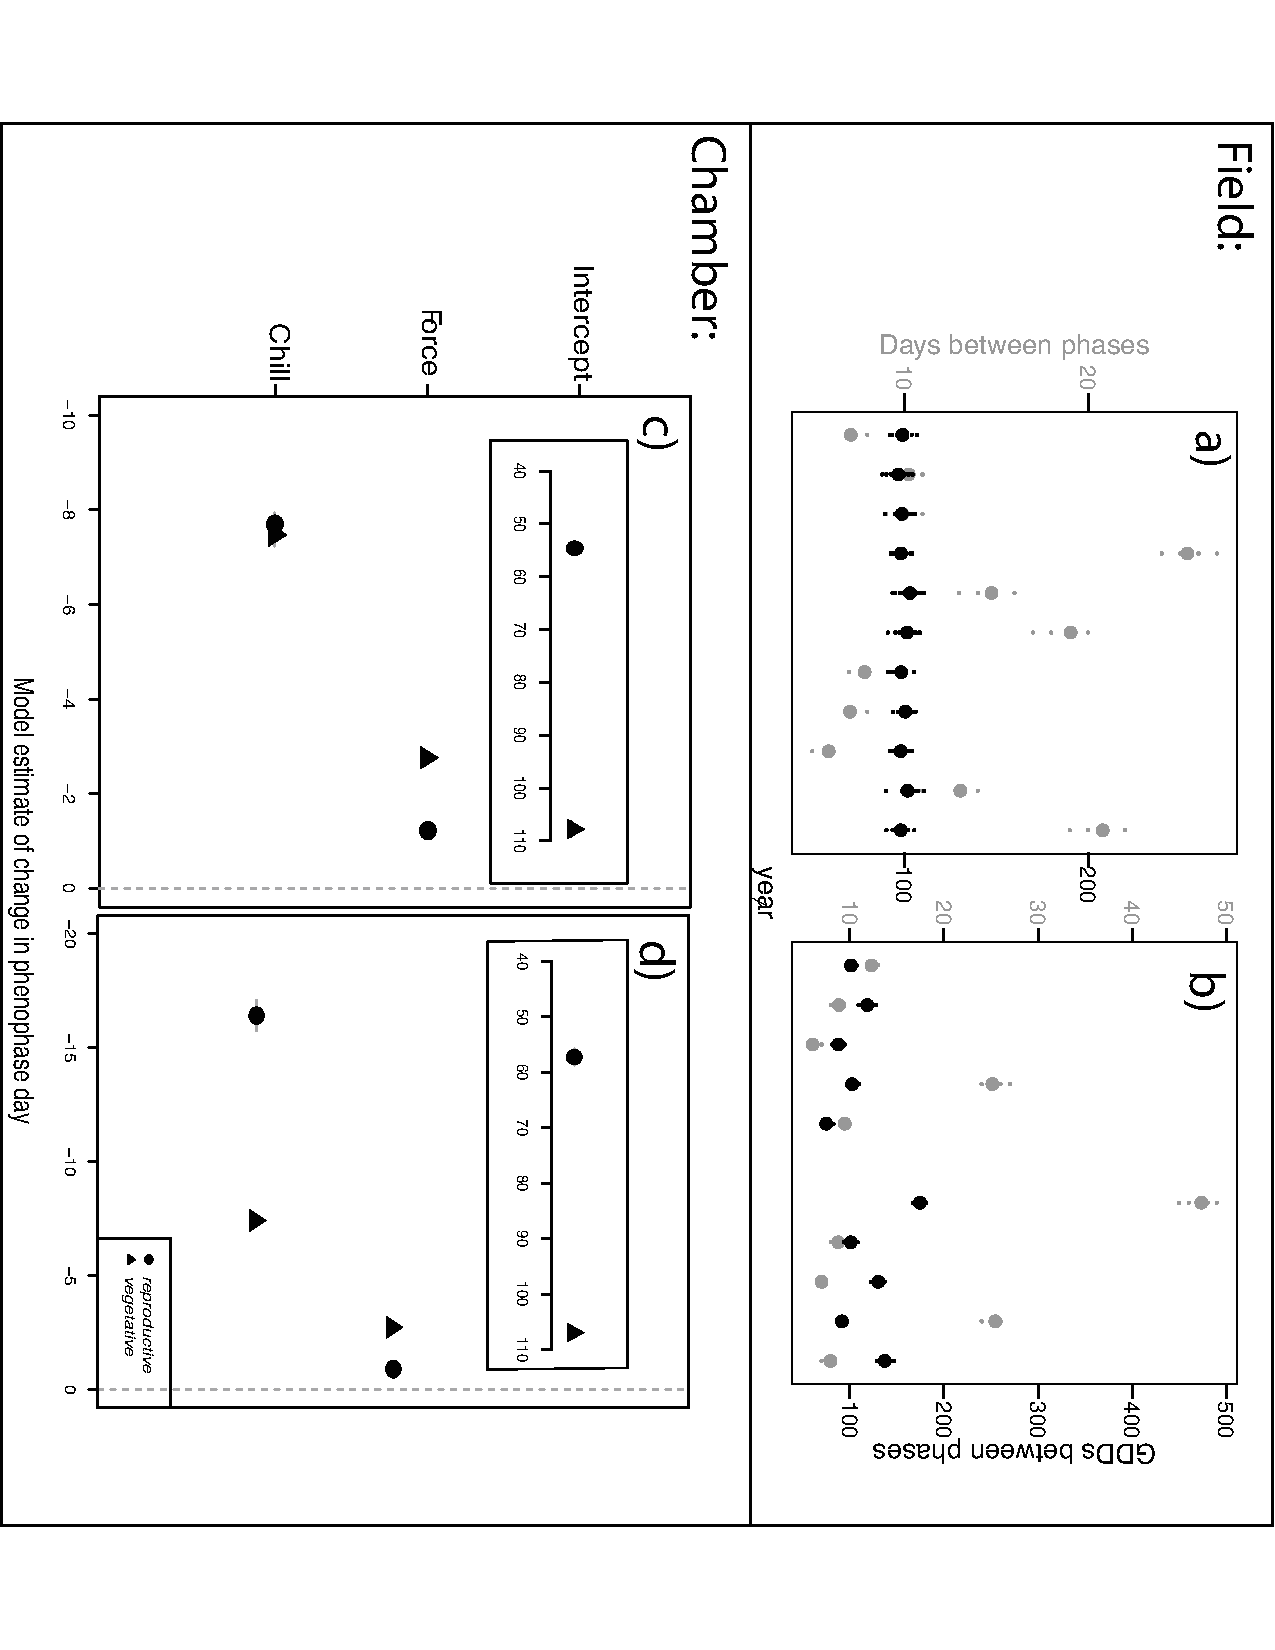
\includegraphics[width=\textwidth]{..//Plots/Flobuds_manuscript_figs/simulationfigure.pdf}
    \label{fig:field}
\end{figure}

\begin{figure}[h!]
    \centering
 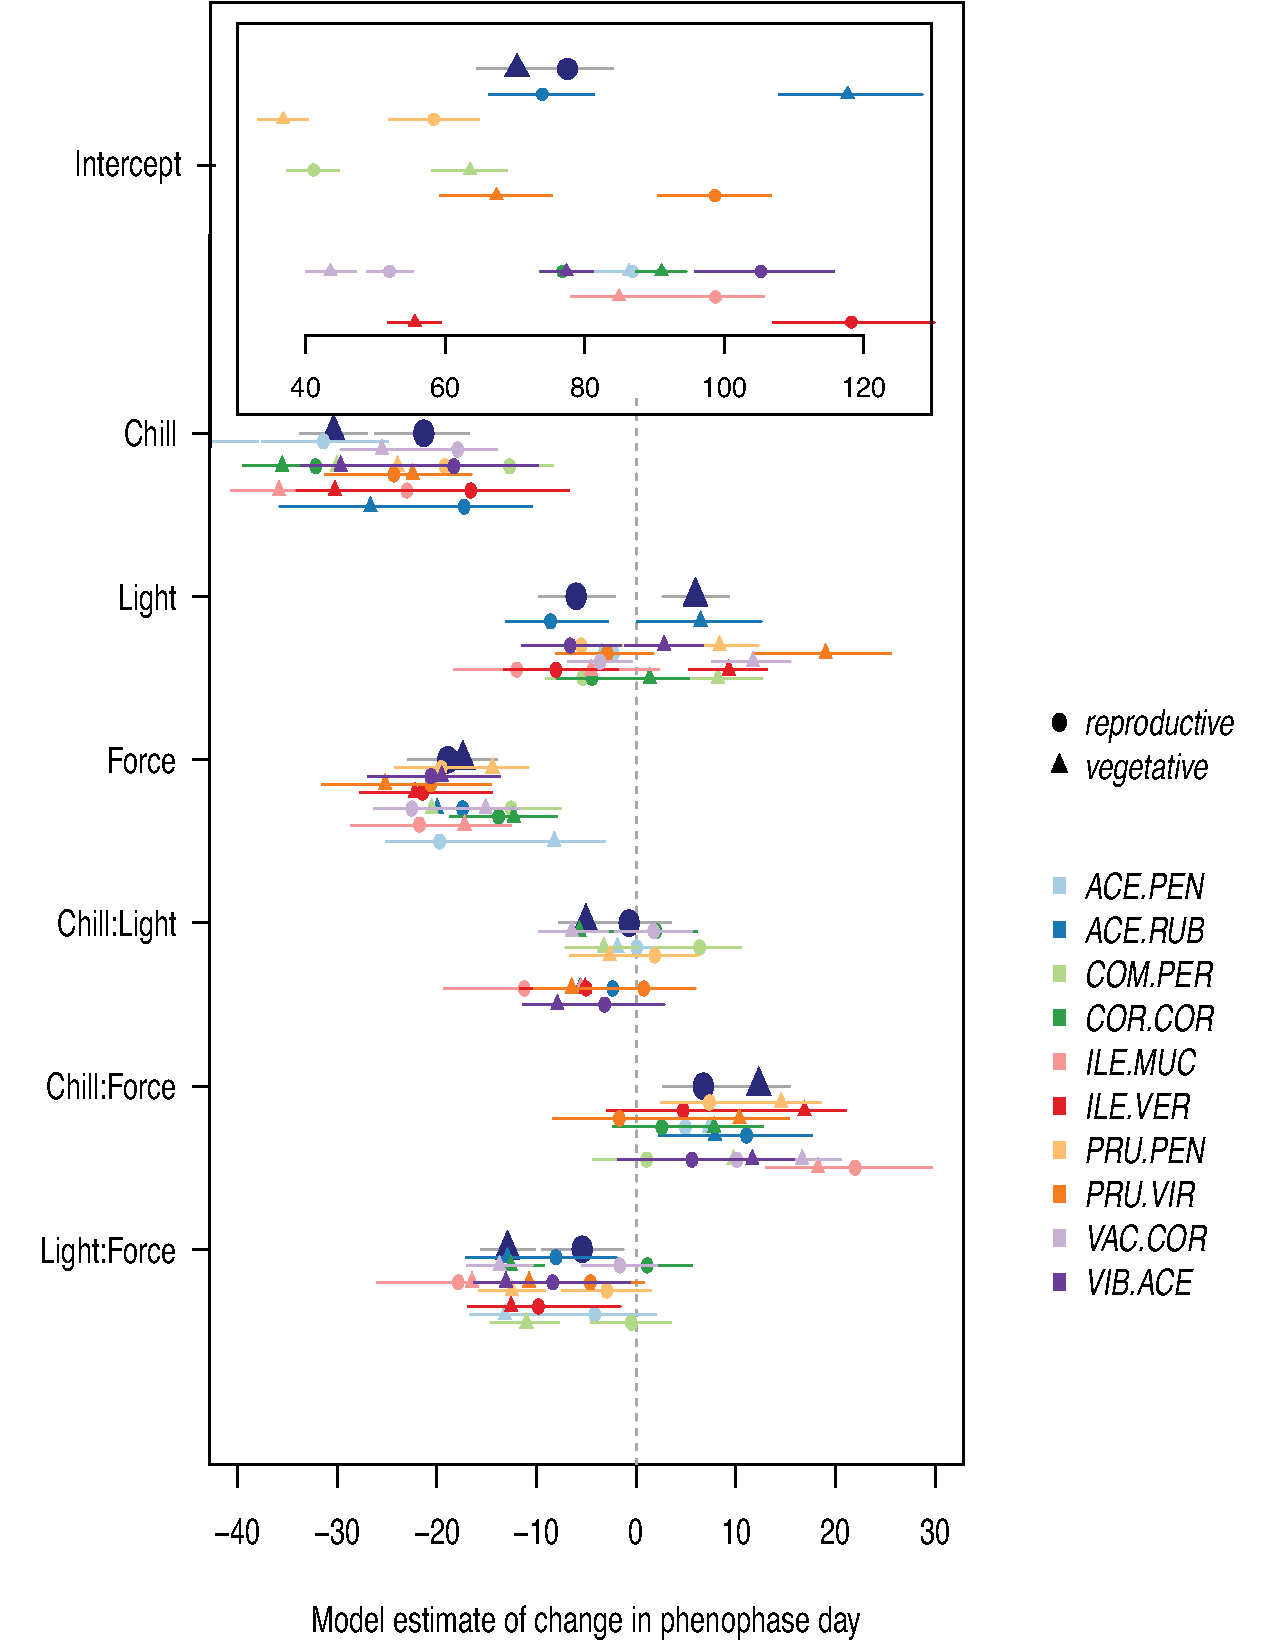
\includegraphics[width=\textwidth]{..//Plots/Flobuds_manuscript_figs/budburstvsflowering.pdf}
    \caption{\textbf{Experimental results suggest differential sensitivity to environmental cues between flower and leaf buds}. Vegetative buds (circles) as more sensitive to chilling and interaction between chilling and forcing. Flower buds (triangles) advance with photoperiods increases but leaf buds appear to delay. These differential sensitivities have implications with how FLS patterns vary given environmental variation}
    \label{fig:model}
\end{figure}


\begin{figure}[h!]
    \centering
 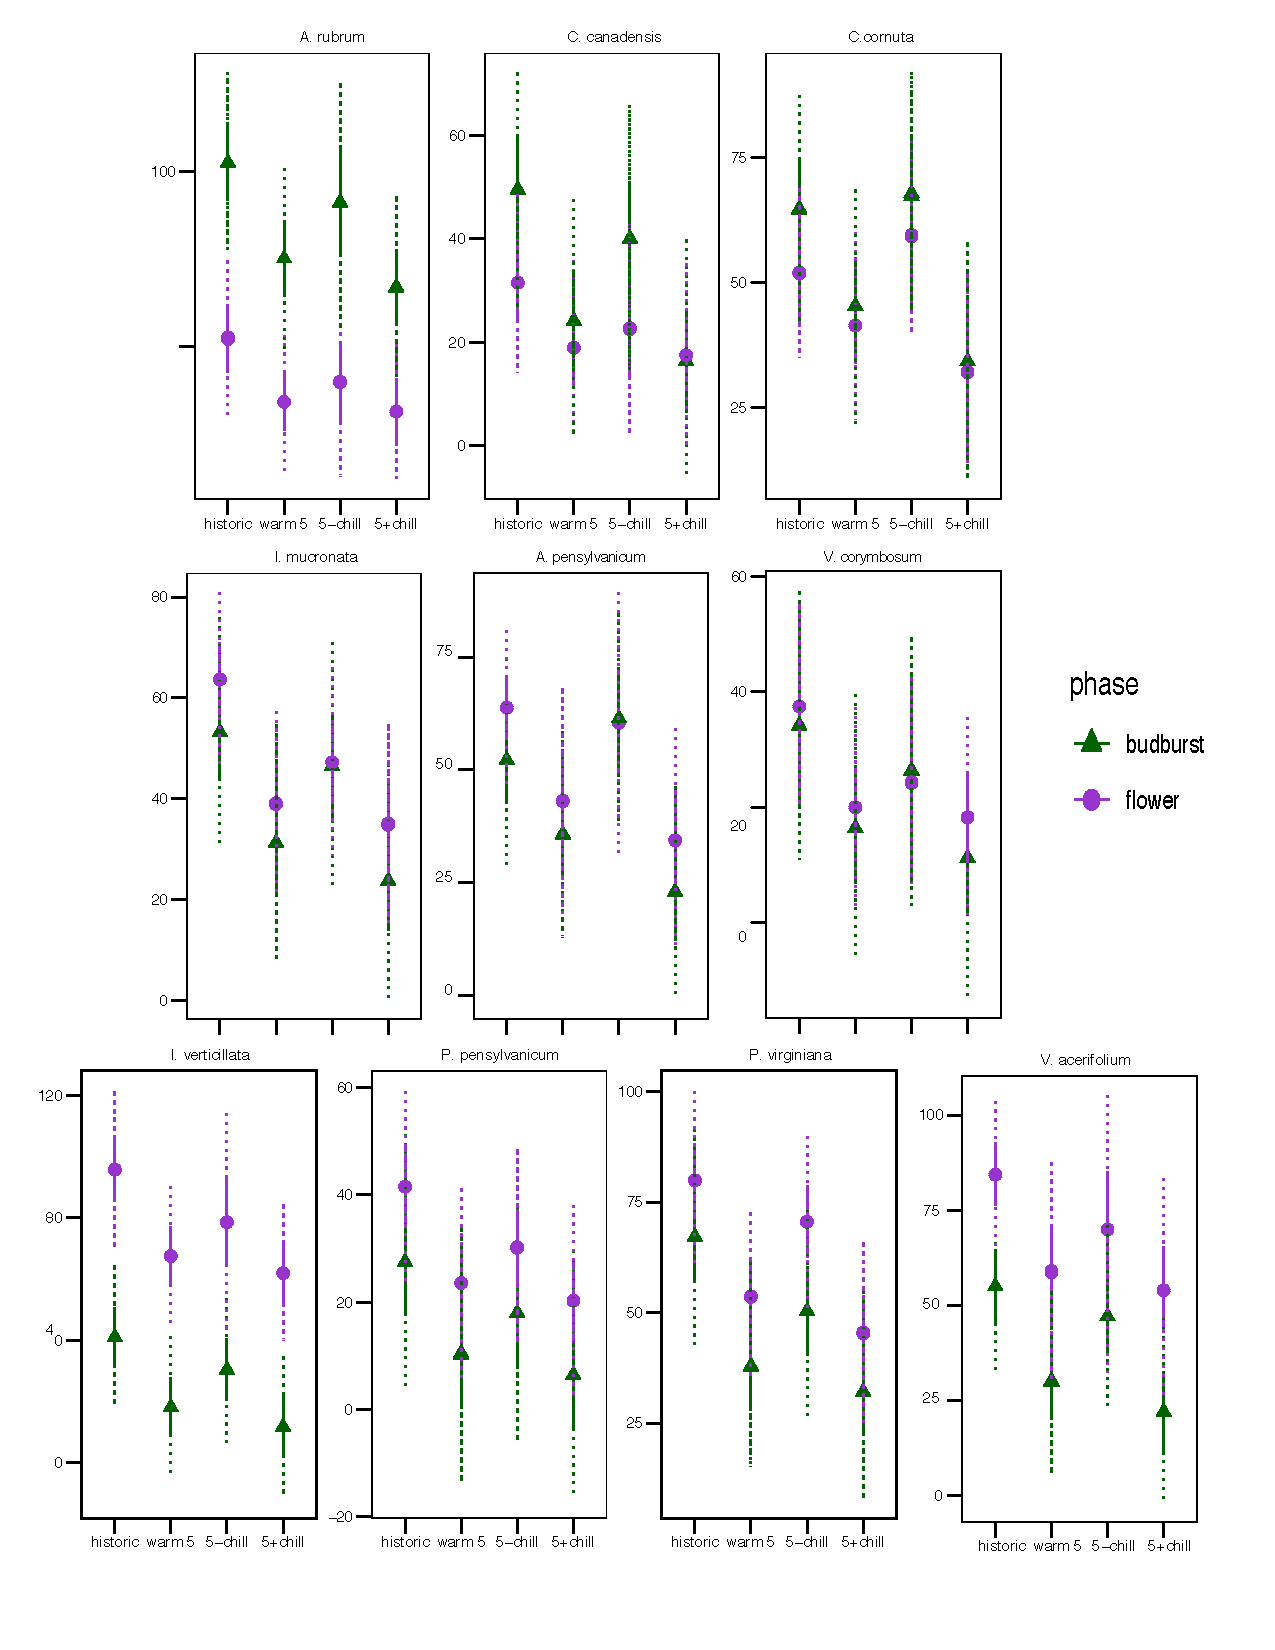
\includegraphics[width=\textwidth]{..//Plots/Flobuds_manuscript_figs/climpredictions.pdf}
    \caption{}
    \label{fig:preddy}
\end{figure}


\end{document}